%
\begin{kd}
	Trong công nghiệp, đơn chất nitrogen kết hợp với hydrogen tạo thành ammonia là một hợp chất quan trọng trong sản xuất phân bón, hoá chất.\\
	Tại sao phản ứng trên cấn thực hiện ở nhiệt độ cao? Đơn chất nitrogen đóng vai trò gì trong phản ứng đó?
\end{kd}
\subsubsection{Trạng thái tự nhiên}
		Nitơ (N) là một nguyên tố hóa học có số hiệu nguyên tử là 7. Đây là một trong những phi kim quan trọng nhất trong tự nhiên và đóng vai trò không thể thiếu trong chu trình sinh địa hóa học.Nitơ tồn tại dưới nhiều dạng và có mặt trong nhiều hệ sinh thái khác nhau, từ khí quyển, đại dương đến các hệ sinh vật sống. Dưới đây là các nguồn phân bố chính của nitơ:
	\clearpage
	\begin{itemize}
		\item \indam[black]{Nitơ trong khí quyển}:
			\begin{paracol}{2}
				\begin{itemize}
					\item Nitơ tồn tại chủ yếu dưới dạng nitơ phân tử (N$_2$), là một chất khí không màu, không mùi.
					\item N$_2$ khá trơ về mặt hóa học do liên kết ba rất bền giữa các nguyên tử nitơ trong phân tử N$_2$.
					\item Khí Nitơ chiếm khoảng 78\% thành phần khí quyển.
				\end{itemize}
				\switchcolumn
				\includegraphics[height=4cm]{Images/anhhoa11/C2_B04_DON_CHAT_NITROGEN/ThanhphanKhongKhi.png}
				\captionof{figure}{Thành phần thể tích\\ của không khí}
			\end{paracol}
		\begin{paracol}{2}
			\item \indam[black]{Nitơ trong sinh vật sống:} 
			\begin{itemize}
				\item Nitơ là thành phần thiết yếu của các axit amin, protein và axit nucleic.
				\item Trong hệ sinh học, Nitơ thường tồn tại dưới dạng amonia (NH$_3$), nitrit (NO$_2^-$), và nitrat (NO$_3^-$).
				\item Nitơ có vai trò quan trọng trong sự phát triển của thực vật và chu trình dinh dưỡng.
			\end{itemize}
			\switchcolumn
			\begin{Bancobiet}[\mycolor]
				\includegraphics[width=5cm,trim={2cm 2cm 0.5cm 2cm},clip]{Images/anhhoa11/C2_B04_DON_CHAT_NITROGEN/HopchatchuaNito.png}
				Arginine là chất thiết yếu cho quá trình tổng hợp protein trong cơ thể.
				Phân tử arginine chứa 4 nguyên tử $N$.
			\end{Bancobiet}
		\end{paracol}
		\begin{paracol}{2}
				\item \indam[black]{Nitơ trong đất:} 
				\begin{itemize}
					\item Nitơ trong đất chủ yếu tồn tại dưới dạng các hợp chất vô cơ như amonia (NH$_3$) và nitrat (NO$_3^-$).
					\item Thực vật hấp thụ nitrat và amonia từ đất để tổng hợp protein và các hợp chất hữu cơ khác.
				\end{itemize}
				\item \indam[black]{Nitơ trong các đại dương:} 
				\begin{itemize}
					\item Đại dương chứa một lượng lớn nitơ, chủ yếu tồn tại dưới dạng các ion nitrat và amonia.
					\item Nitơ đóng vai trò quan trọng trong hệ sinh thái biển, hỗ trợ sự phát triển của sinh vật phù du và các sinh vật khác.
				\end{itemize}
				\switchcolumn
				\includegraphics[width=5cm]{Images/anhhoa11/C2_B04_DON_CHAT_NITROGEN/ChutrinhNitrogen.png}
		\end{paracol}
	\end{itemize}
\subsubsection{Cấu tạo nguyên tử, phân tử}
	\Noibat[][]{Cấu tạo nguyên tử}
	\begin{hopdongian}
		\hinhphai{Nguyên tố nitrogen ở ô số 7 , nhóm VA, chu kì 2 trong bảng tuần hoàn. Nguyên tử nitrogen có độ âm điện lớn $(3,04)$. Nitrogen là phi kim điển hình.\\
		Nitrogen tạo ra nhiều hợp chất với các số oxi hoá khác nhau từ -3 đến +5 . Các số oxi hoá thường gặp của nitrogen được biểu diễn ở trục số oxi hoá dưới đây.\\
		\begin{tikzpicture}[declare function={r=3;},line cap=round,line join=round]
			\foreach \x [count=\i from 1] in {-3,0,1,2,3,4,5}{%
				\path (\x,0) node [inner sep=0pt,outer sep =0pt,anchor =center] (d-\i){%
					\tikz{%
						\draw[line width=1pt,\maunhan](0,0) --(0,4pt);
					}
				};
				\path (d-\i.north) node [anchor=south,text=\maudam,font=\bfseries\sffamily\scriptsize] {%
					\ifnum\x>0
					+\x
					\else
					\x
					\fi
				};
			}
			\draw[->,-stealth,line width=0.8pt](-3.5,0)--(5.5,0);
			\path (d-2.south) node [anchor=north,text=\maunhan,font=\large] {$\mathsf{N_2}$};
		\end{tikzpicture}
		}{%
			\includegraphics[width=4cm]{Images/anhhoa11/C2_B04_DON_CHAT_NITROGEN/SodocautaoNito.png}
		}
	\end{hopdongian}
	\begin{hoivadap}
		\begin{enumerate}
			\item Sắp xếp các hợp chất sau vào vị trí tương ứng trong trục biểu diễn số oxi hoá của nitrogen: $\mathrm{NO}, \mathrm{N}_2 \mathrm{O}, \mathrm{NO}_2, \mathrm{NH}_3, \mathrm{HNO}_2, \mathrm{HNO}_3, \mathrm{NH}_4 \mathrm{Cl}, \mathrm{KNO}_2, \mathrm{NaNO}_3$.
			\item Dựa vào trục biểu diễn số oxi hoá của nitrogen để giải thích nitrogen có cả tính oxi hoá và tính khử. Viết một quá trình oxi hoá và một quá trình khử để minh hoạ.
		\end{enumerate}
		\loigiai{
		\begin{enumerate}
			\item \begin{tikzpicture}[declare function={r=3;hs=1.5;},line cap=round,line join=round, baseline]
				\foreach \x [count=\i from 1] in {-3,0,1,2,3,4,5}{%
					\path (\x*hs,0) node [inner sep=0pt,outer sep =0pt,anchor =center] (d-\i){%
						\tikz{%
							\draw[line width=1pt,\maunhan](0,0) --(0,4pt);
						}
					};
					\path (d-\i.north) node [anchor=south,text=\maudam,font=\bfseries\sffamily\scriptsize] {%
						\ifnum\x>0
						+\x
						\else
						\x
						\fi
					};
				}
				\draw[->,-stealth,line width=0.8pt](-3.5*hs,0)--(5.5*hs,0);
				\foreach \x/\n in {%
					1/{$NH_3$, $NH_4Cl$},3/$N_2O$,
					4/$NO$,5/{$HNO_2$, $KNO_2$},
					6/{$NO_2$},7/{$HNO_3$, $NaNO_3$}
					}{
					\path (d-\x.south) node [anchor=north,text=\maunhan,font=\scriptsize,fill=\maunhan!15,inner sep=4pt, outer sep =2pt,rounded corners =3pt] {\n};
				}
				\path (d-2.south) node [anchor=north,text=\maudam,font=\large,fill=\maudam!15,inner sep=4pt, outer sep =2pt,rounded corners =3pt] {$\mathsf{N_2}$};
			\end{tikzpicture}
			\item $N_2$ có số oxi-hóa bằng $0$ là số oxi hóa trung gian nên khi tham gia phản ứng hóa học $N_2$ sẽ có 2 khuynh hướng:
			\begin{itemize}
				\item giảm số oxi-hóa từ $0$ xuống $-3$ thể hiện tính oxi hóa:
				\textbf{Ví dụ:}  $N_2$ $+$ $H_2$ $\xleftrightarrow$ $NH_3$
				\item tăng số oxi-hóa từ $0$ lên $+1$, $+2$, $+3$, $+4$, $+5$ thể hiện tính khử:\textbf{Ví dụ:}  $N_2$ $+$ $O_2$ $\xrightarrow[$3000^\circ C$][][1.5]$ $2NO$
			\end{itemize}
		\end{enumerate}
		}
	\end{hoivadap}
	\Noibat[][]{Cấu tạo phân tử}
	\immini{Phân tử nitrogen gồm hai nguyên tử, liên kết với nhau bằng liên kết ba ( 1 liên kết $\sigma$ và 2 liên kết $\pi)$. Phân tử nitrogen có năng lượng liên kết lớn $(945 \mathrm{~kJ} / \mathrm{mol})$ và không có cực.}{
		\includegraphics[width=5cm]{Images/anhhoa11/C2_B04_DON_CHAT_NITROGEN/CautaoPTNito.png}
	}
	\begin{hoivadap}
		\begin{enumerate}
			\item Viết công thức electron, công thức Lewis và công thức cấu tạo của phân tử nitrogen.
			\item Từ cấu tạo phân tử, hãy cho biết tại sao phân tử $N_2$ có năng lượng liên kết lớn. Dự đoán về khả năng hoạt động hoá học của nitrogen ở nhiệt độ thường.
		\end{enumerate}
		\loigiai{%
		\begin{enumerate}
			\item \begin{tabular}{C{0.2\linewidth}C{0.2\linewidth}C{0.2\linewidth}}
			Công thức electron&Công thức Lewis&Công thức cấu tạo\\
			\chemfig[atom sep=2em]{\charge{90:2pt=\:,0:2pt=\.,0:2pt=\.[{.style={yshift=2.65mm,fill=black}}],0:2pt=\.[{.style={yshift=-2.65mm,fill=black}}]}{N}-[,0.85,,,draw=none]\charge{90:2pt=\:,180:2pt=\.,180:2pt=\.[{.style={yshift=2.65mm,fill=black}}],180:2pt=\.[{.style={yshift=-2.65mm,fill=black}}]}{N}}&\chemfig[atom sep=2em]{\charge{90:2pt=\:}{N}~\charge{90:2pt=\:}{N}}&\chemfig[atom sep=2em]{N~N}
			\end{tabular}
			\item Do trong cấu tạo có liên kết ba bền vững nên năng lượng liên kết rất lớn vì thế ở nhiệt độ thường phân tử $N_2$ khá trơ về mặt hóa học.
		\end{enumerate}
		}
	\end{hoivadap}
\subsubsection{Tính chất vật lý}
	\begin{ghinho}
		\Rightpicture[0.65]{Ở điều kiện thường, nitrogen là chất khí, không màu, không mùi, không vị, khó hoá lỏng (hoá lỏng ở $-196^{\circ} \mathrm{C}$ ), tan rất ít trong nước (1 lít nước hoà tan được 0{,}012 lít khí nitrogen). Khí nitrogen không duy trì sự cháy và sự hô hấp.}{\includegraphics[width=5cm]{Images/anhhoa11/C2_B04_DON_CHAT_NITROGEN/Liquid_Nitrogen.png}}
	\end{ghinho}
	\begin{hoivadap}
		\begin{enumerate}
			\item Dựa vào tương tác van der Waals, hãy giải thích tại sao đơn chất $\mathrm{N}_2$ khó hoá lỏng và ít tan trong nước.
		\end{enumerate}
		\loigiai{
		\begin{itemize}
			\item Do phân tử $N_2$ không phân cực, khối lượng nhỏ  nên lực tương tác van der Waals giữa các phân tử với nhau rất nhỏ dẫn đến lực hút giữa các phân tử  không thể vượt qua động năng lúc này các phân tử dễ dàng chuyển động ra xa nhau , duy trì trạng thái khí.
			\item Vì $N_2$ là phân tử phân cực trong khi đó $H_2O$ là một phân tử phân cực nên tương tác van der Waals giữa $H_2O$ và $N_2$ yếu nên $N_2$ ít tan trong nước.
		\end{itemize}
			}
	\end{hoivadap}
\subsubsection{Tính chất hóa học}
\Noibat[][]{Tác dụng với hydrogen}
 $\mathrm{N}_2(\mathrm{g})+3 \mathrm{H}_2(\mathrm{g}) \xharpoonarrow[$400 - 600 ^\circ$][$200~bar, Fe$][2] 2 \mathrm{NH}_3(\mathrm{g})$ $\Delta_{\mathrm{r}} \mathrm{H}_{298}^{\circ}=-91{,}8 \mathrm{~kJ}$
 \Noibat[][]{Tác dụng với Oxygen}
 $ \mathrm{N}_2(g) + O_2(g) \xharpoonarrow[$3000^\circ$] 2NO(g) \qquad \Delta_r H^{\circ}_{298} = 182,6 \, \text{kJ} $
 \Noibat[][]{Quá trình tạo và cung cấp nitrate cho đất từ nước mưa}
 \begin{center}
 	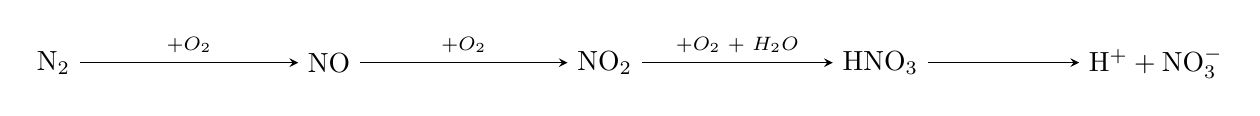
\begin{tikzpicture}[declare function={d=3.5 cm;},>=stealth]
 		\path (0,0)  node (N2) {$\mathrm{N}_2$}
 		 --++(d,0)  node (NO) {$\mathrm{NO}$}
 		 --++(d,0) node (NO2) {$\mathrm{NO}_2$}
 		 --++(d,0)  node (HNO3) {$\mathrm{HNO}_3$}
 		 --++(d,0)  node (NO3) {$\mathrm{H}^+ + \mathrm{NO}_3^-$}
 		;
 		\foreach \x/\y/\n in {%
 			N2/NO/+$O_2$, NO/NO2/+$O_2$,
 			NO2/HNO3/+$O_2$ + $H_2O$,HNO3/NO3/\phantom{x}
 		}{%
 		\draw[->] (\x.east)--(\y.west) node [above,sloped, pos=0.5,font=\scriptsize]{\n} ;
 		}%
 	\end{tikzpicture}
 \end{center}
 \begin{hoivadap}
 	Sử dụng kiến thức hóa học giải thích câu ca dao sau:
 	\begin{center}
 		\lq\lq Lúa chiêm lấp ló đầu bờ\\
 		Hễ nghe tiếng sấm phất cờ mà lên
 		\rq\rq\\
 		\includegraphics[width=5cm]{Images/anhhoa11/C2_B04_DON_CHAT_NITROGEN/luachiem.png}
 	\end{center}
 	\loigiai{
 	Hiện tượng "Lúa chiêm lấp ló đầu bờ, hễ nghe tiếng sấm phất cờ mà lên" được giải thích dựa trên quá trình \textbf{cố định đạm tự nhiên} trong khí quyển nhờ sấm sét.
 	
 	Trong không khí, có khoảng 78\% là khí nitơ ($N_2$). Mặc dù là một nguyên tố dinh dưỡng cực kỳ quan trọng cho cây trồng, nitơ ở dạng phân tử ($N_2$) rất trơ và cây không thể hấp thụ trực tiếp được. Khi có sấm sét, năng lượng khổng lồ từ tia lửa điện cung cấp đủ năng lượng để phá vỡ liên kết ba bền vững trong phân tử nitơ, giúp nó phản ứng với oxy trong không khí.
 	
 	Quá trình này diễn ra qua các bước sau:
 	
 	\begin{enumerate}
 		\item \textbf{Nitơ tác dụng với oxy tạo Nitơ monooxit (NO):} \\
 		Năng lượng cực lớn từ tia sét "đốt cháy" nitơ trong không khí.
 		\[\mathrm{N}_2 + \mathrm{O}_2 \xrightarrow[$\text{tia lửa điện}$] 2\mathrm{NO}\]
 		\item \textbf{Oxi hóa Nitơ monooxit (NO) thành Nitơ đioxit ($NO_2$):} \\
 		Khí NO sinh ra không bền và nhanh chóng phản ứng với oxy trong không khí tạo thành $NO_2$, một khí có màu nâu đỏ.
 		\[2\mathrm{NO} + \mathrm{O}_2 \xrightarrow 2\mathrm{NO}_2\]
 		\item \textbf{$NO_2$ phản ứng với nước mưa tạo axit nitric ($HNO_3$):} \\
 		Khí $NO_2$ hòa tan trong nước mưa và tác dụng với oxy trong không khí để tạo thành axit nitric.
 		\[4\mathrm{NO}_2 + \mathrm{O}_2 + 2\mathrm{H}_2\mathrm{O} \xrightarrow 4\mathrm{HNO}_3\]
 		\item \textbf{Axit nitric theo nước mưa rơi xuống đất và tạo muối nitrat:} \\
 		Axit nitric ($HNO_3$) theo mưa rơi xuống đất sẽ phản ứng với các khoáng chất có tính bazơ trong đất để tạo thành muối \textbf{nitrat ($NO_3^-$)}. Đây chính là dạng "phân đạm" mà rễ cây lúa có thể hấp thụ dễ dàng.
 		\[\mathrm{HNO}_3 + \text{chất bazơ trong đất} \xrightarrow \text{Muối Nitrat} + \mathrm{H}_2\mathrm{O}\]
 	\end{enumerate}
 	\textbf{Kết luận:} Nhờ có sấm sét, một lượng lớn đạm tự nhiên từ không khí đã được chuyển hóa thành dạng dinh dưỡng dễ tiêu cho cây lúa. Lượng "phân đạm trời cho" này giúp cây lúa, đặc biệt là lúa chiêm đang trong giai đoạn sinh trưởng mạnh, phát triển nhanh chóng, vươn cao, tượng trưng cho hình ảnh "phất cờ mà lên".
 	}
 \end{hoivadap}
 \begin{ghinho}
 	Ở nhiệt độ thường, phân tử nitrogen rất bền, khá trơ về mặt hoá học. Trong các điều kiện thích hợp, nitrogen chủ yếu thể hiện tính oxi hoá, nitrogen thể hiện tính khử khi tác dụng với oxygen.
 \end{ghinho}
 \begin{hoivadap}
 \begin{enumerate}
 	\item  Trong phương trình hoá học của phản ứng tổng hợp ammonia, hãy xác định các nguyên tử có sự thay đổi số oxi hoá và vai trò của nitrogen.
 	\item Trong phương trình hoá học của phản ứng giữa nitrogen với oxygen:
 	\begin{enumerate}[a)]
 		\item Hãy xác định các nguyên tử có sự thay đổi số oxi hoá.
 		\item Tại sao thực tế không sử dụng phản ứng này để tạo ra NO, một hợp chất trung gian quan trọng trong công nghiệp sản xuất nitric acid?
 	\end{enumerate}
 	\item Viết các phương trình hoá học minh hoạ quá trình hình thành đạm nitrate trong tự nhiên xuất phát từ nitrogen.
 \end{enumerate}
 \loigiai{
 \begin{enumerate}
 	\item Phương trình hóa học của phản ứng tổng hợp ammonia (quá trình Haber-Bosch):
 	\[ \mathrm{N}_2 + 3\mathrm{H}_2 \xharpoonarrow 2\mathrm{NH}_3 \]
 	\begin{itemize}
 		\item Sự thay đổi số oxi hóa:
 		\begin{itemize}
 			\item \textbf{Nitrogen (N):} Số oxi hóa giảm từ \textbf{0} (trong $N_2$) xuống \textbf{-3} (trong $NH_3$).
 			\item \textbf{Hydrogen (H):} Số oxi hóa tăng từ \textbf{0} (trong $H_2$) lên \textbf{+1} (trong $NH_3$).
 		\end{itemize}
 		\item \textbf{Vai trò của Nitrogen:} Do số oxi hóa giảm (nhận electron), nitrogen đóng vai trò là \textbf{chất oxi hóa}.
 	\end{itemize}
 	\item Trong phương trình hoá học của phản ứng giữa nitrogen với oxygen:
 	Phương trình hóa học:
 	\[ \mathrm{N}_2 + \mathrm{O}_2 \xharpoonarrow 2\mathrm{NO} \]
 	\begin{enumerate}[a)]
 		\item \textbf{Hãy xác định các nguyên tử có sự thay đổi số oxi hoá.}
 		\begin{itemize}
 			\item \textbf{Nitrogen (N):} Số oxi hóa tăng từ \textbf{0} (trong $N_2$) lên \textbf{+2} (trong NO).
 			\item \textbf{Oxygen (O):} Số oxi hóa giảm từ \textbf{0} (trong $O_2$) xuống \textbf{-2} (trong NO).
 		\end{itemize}
 		\item Tại sao thực tế không sử dụng phản ứng này để tạo ra NO?
 		Phản ứng này không được sử dụng trong công nghiệp vì:
 		\begin{itemize}
 			\item Điều kiện khắc nghiệt: Phản ứng yêu cầu nhiệt độ rất cao ($\sim 3000^\circ C$), gây tốn kém năng lượng.
 			\item Hiệu suất thấp: Phản ứng là thuận nghịch và có hiệu suất rất thấp, không kinh tế.
 			\item Có phương pháp hiệu quả hơn: Công nghiệp sử dụng quá trình Ostwald để oxi hóa $NH_3$ với hiệu suất cao hơn:
 			\[ 4\mathrm{NH}_3 + 5\mathrm{O}_2 \xrightarrow[$Pt, t^\circ$] 4\mathrm{NO} + 6\mathrm{H}_2\mathrm{O} \]
 		\end{itemize}
 	\end{enumerate}
 	\item Viết các phương trình hoá học minh hoạ quá trình hình thành đạm nitrate trong tự nhiên xuất phát từ nitrogen.
	Quá trình hình thành đạm nitrate ($NO_3^-$) trong tự nhiên từ $N_2$ khí quyển (nhờ sấm sét) diễn ra qua các bước:
 	\begin{enumerate}[a)]
 		\item Nitrogen phản ứng với oxygen tạo thành nitric oxide:
 		\[ \mathrm{N}_2 + \mathrm{O}_2 \xrightarrow[$\text{tia lửa điện}$] 2\mathrm{NO} \]
 		\item Nitric oxide bị oxi hóa thành nitrogen dioxide:
 		\[ 2\mathrm{NO} + \mathrm{O}_2 \xrightarrow 2\mathrm{NO}_2 \]
 		\item Nitrogen dioxide phản ứng với oxygen và nước tạo nitric acid:
 		\[ 4\mathrm{NO}_2 + \mathrm{O}_2 + 2\mathrm{H}_2\mathrm{O} \xrightarrow 4\mathrm{HNO}_3 \]
 		\item Nitric acid theo mưa rơi xuống đất và tạo thành muối nitrate ($NO_3^-$), cung cấp đạm cho thực vật.
 	\end{enumerate}
 \end{enumerate}
 }
 \end{hoivadap}
 \begin{Bancobiet}
 	Một số vi sinh vật chuyển hoá nitrogen thành phân đạm, tích luỹ tại các nốt sần ở rễ cây họ đậu. Quá trình này góp phần cải tạo và bổ sung dinh dưỡng cho đất trồng.
 	\begin{center}
 		\includegraphics[width=5cm]{Images/anhhoa11/C2_B04_DON_CHAT_NITROGEN/em_co_biet_not_san_ho_dau.png}
 	\end{center}
 	\captionof{figure}{Nốt sần ở rễ cây cây đậu}
 \end{Bancobiet}
\subsubsection{Ứng dụng}
%%%lệnh vẽ mũi tên
\newcommand{\muiten}{
	\begin{tikzpicture}[declare function={d=1.8cm;}]
		\path (0,0)  coordinate (A)
		(d,0)  coordinate (B)
		($(A)+(90:6pt)$) coordinate (At)
		($(B)+(90:6pt)+(-0.5cm,0)$) coordinate (Bt)
		($(Bt)+(90:5pt)$) coordinate (Btt)
		($(A)+(-90:6pt)$) coordinate (Ath)
		($(B)+(-90:6pt)+(-0.5cm,0)$) coordinate (Bth)
		($(Bth)+(-90:5pt)$) coordinate (Btth)
		;
		\path [fill=\mycolor!75] (At)--(Bt)--(Btt)--(B)--(Btth)--(Bth)--(Ath)--cycle;
	\end{tikzpicture}
}
\begin{center}
	\begin{tikzpicture}[declare function ={r=1.3cm;}]
		%%Vẽ node tròn nền đậm
		\path (0,0) node (tempt) [circle,align=center,rounded corners=6pt, fill=\mycolor!60,font=\sffamily\bfseries, text width = 3cm,inner sep =2pt,minimum size=3.6cm]{};
		%%Vẽ node tròn tiêu đề chính
		\path (0,0) node (brain) [circle,align=center,rounded corners=6pt, fill=\mycolor!20,font=\sffamily\bfseries, text width = 3cm,inner sep =2pt,minimum size=3.1cm]{Ứng dụng của\\ nitrogen};
		%%Vẽ mũi tên và hình ảnh minh họa
		\foreach [count=\i] \g/\n/\p/\m/\c in {
			18/Bao_quan_thuc_pham.png/north/south/Bảo quản thực phẩm,%
			90/Duoc_pham.png/north/south/Dược phẩm,%
			162/Phan_bon.png/north/south/Phân bón,%
			234/Bao_quan_mau.png/south/north/Tạo môi trường trơ,%
			306/bao_quan_lanh.png/south/north/Bảo quản lạnh%
		}{
			\path ($(brain)+(\g:2.8cm)$) node (ud\i)[rotate=\g] {\muiten};
			\draw ($(ud\i)+(\g:2.25cm)$) circle (r);
			\begin{scope}
				\clip ($(ud\i)+ (\g:2.25cm)$) circle (r);
				\path ($(ud\i)+ (\g:2.25cm)$) node (images\i) {\includegraphics[width=2.6cm]{Images/anhhoa11/C2_B04_DON_CHAT_NITROGEN/\n}};
			\end{scope}
			\path (images\i.\p) node[text width =2.5cm, anchor=\m,align=center, font=\sffamily\bfseries] {\c};
		}

	\end{tikzpicture}
\end{center}